%!TEX program = xelatex

\documentclass[a4paper, openany, oneside]{memoir}
\usepackage[no-math]{fontspec}
\usepackage{pgfplots}
\pgfplotsset{compat=newest}
\usepackage{commath}
\usepackage{mathtools}
\usepackage{amssymb}
\usepackage{amsthm}
\usepackage{booktabs}
\usepackage{mathtools}
\usepackage{xcolor}
\usepackage[separate-uncertainty=true, per-mode=symbol]{siunitx}
\usepackage[noabbrev, capitalize]{cleveref}
\usepackage{listings}
\usepackage[american inductor, european resistor]{circuitikz}
\usepackage{amsmath}
\usepackage{amsfonts}
\usepackage{ifxetex}
\usepackage[dutch,english]{babel}
\usepackage[backend=bibtexu,texencoding=utf8,bibencoding=utf8,style=ieee,sortlocale=en_GB,language=auto]{biblatex}
\usepackage[strict,autostyle]{csquotes}
\usepackage{parskip}
\usepackage{import}
\usepackage{standalone}
\usepackage{hyperref}
%\usepackage[toc,title,titletoc]{appendix}

\ifxetex{} % Fonts laden in het geval dat je met Xetex compiled
    \usepackage{fontspec}
    \defaultfontfeatures{Ligatures=TeX} % To support LaTeX quoting style
    \setromanfont{Palatino Linotype} % Tover ergens in Font mapje in root.
    \setmonofont{Source Code Pro}
\else % Terug val in standaard pdflatex tool chain. Geen ondersteuning voor OTT fonts
    \usepackage[T1]{fontenc}
    \usepackage[utf8]{inputenc}
\fi
\newcommand{\references}[1]{\begin{flushright}{#1}\end{flushright}}
\renewcommand{\vec}[1]{\boldsymbol{\mathbf{#1}}}
\newcommand{\uvec}[1]{\boldsymbol{\hat{\vec{#1}}}}
\newcommand{\mat}[1]{\boldsymbol{\mathbf{#1}}}
\newcommand{\fasor}[1]{\boldsymbol{\tilde{\vec{#1}}}}
\newcommand{\cmplx}[0]{\mathrm{j}}
\renewcommand{\Re}[0]{\operatorname{Re}}
\newcommand{\Cov}{\operatorname{Cov}}
\newcommand{\Var}{\operatorname{Var}}
\newcommand{\proj}{\operatorname{proj}}
\newcommand{\Perp}{\operatorname{perp}}
\newcommand{\col}{\operatorname{col}}
\newcommand{\rect}{\operatorname{rect}}
\newcommand{\sinc}{\operatorname{sinc}}
\newcommand{\IT}{\operatorname{IT}}
\newcommand{\F}{\mathcal{F}}

\newtheorem{definition}{Definition}
\newtheorem{theorem}{Theorem}


\DeclareSIUnit{\voltampere}{VA} %apparent power
\DeclareSIUnit{\pii}{\ensuremath{\pi}}

\hypersetup{%setup hyperlinks
    colorlinks,
    citecolor=black,
    filecolor=black,
    linkcolor=black,
    urlcolor=black
}

% Example boxes
\usepackage{fancybox}
\usepackage{framed}
\usepackage{adjustbox}
\newenvironment{simpages}%
{\AtBeginEnvironment{itemize}{\parskip=0pt\parsep=0pt\partopsep=0pt}
\def\FrameCommand{\fboxsep=.5\FrameSep\shadowbox}\MakeFramed{\FrameRestore}}%
{\endMakeFramed}

% Impulse train
\DeclareFontFamily{U}{wncy}{}
\DeclareFontShape{U}{wncy}{m}{n}{<->wncyr10}{}
\DeclareSymbolFont{mcy}{U}{wncy}{m}{n}
\DeclareMathSymbol{\Sha}{\mathord}{mcy}{"58}

\pagenumbering{gobble}
% \usetikzlibrary{external}
% \tikzexternalize
% \tikzset{external/system call={xelatex \tikzexternalcheckshellescape
%     -halt-on-error -interaction=batchmode --shell-esape
%     -jobname "\image" "\texsource"}}

\begin{document}

\centerline{
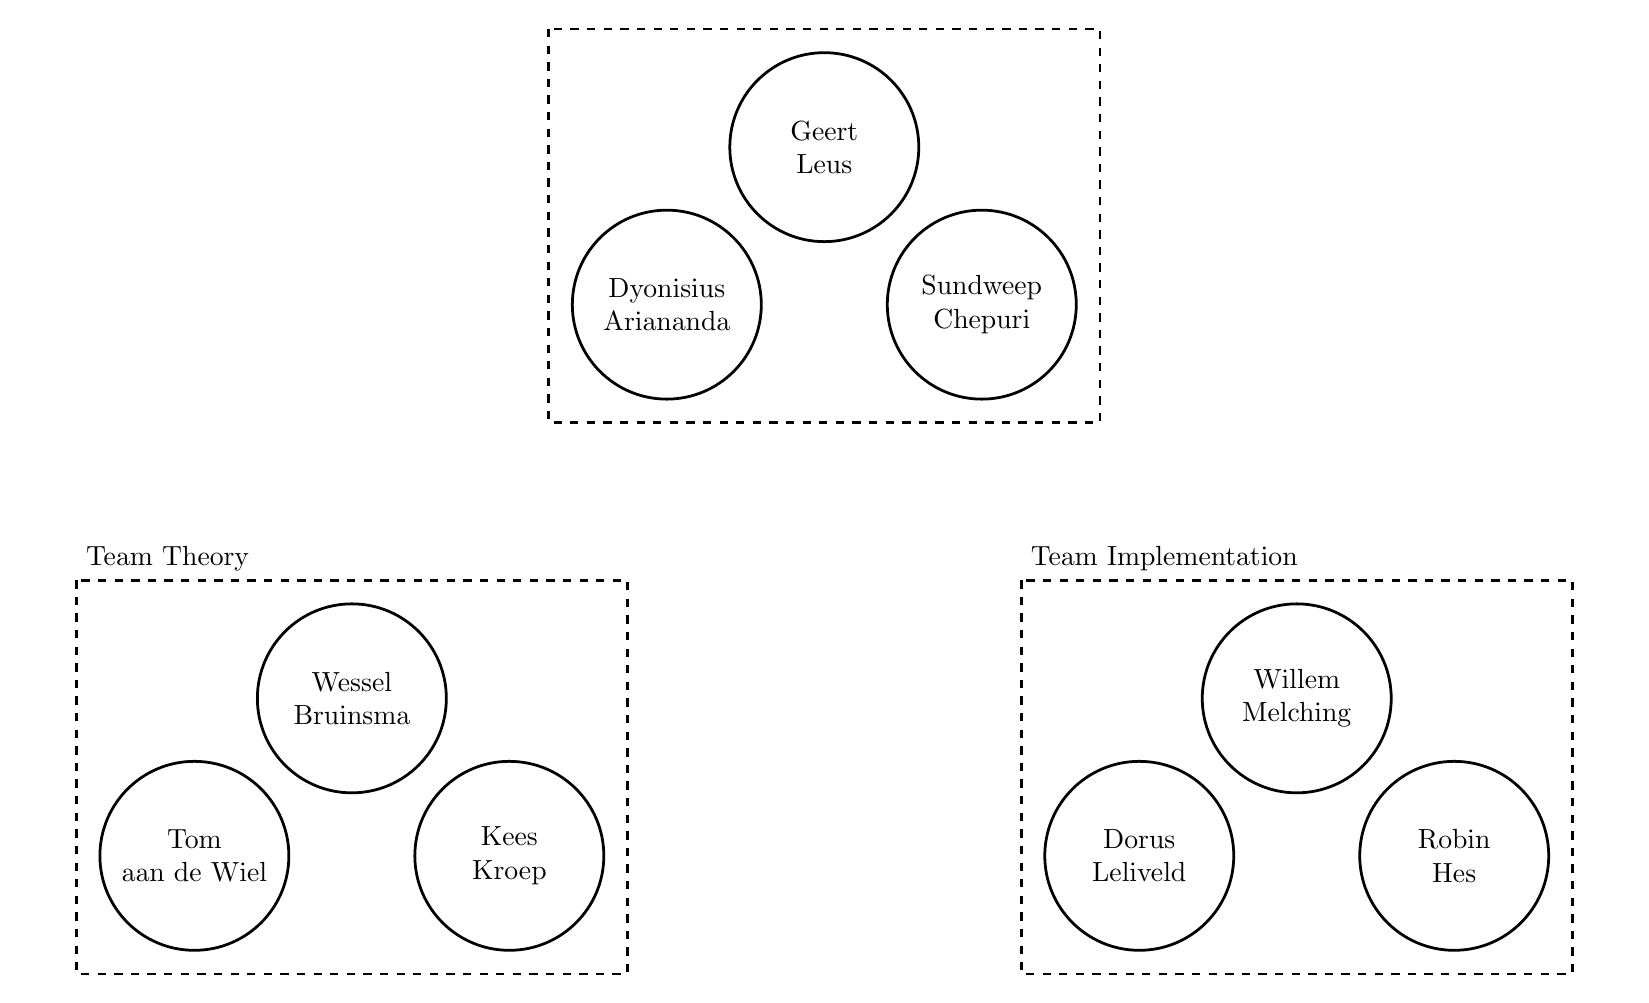
\begin{tikzpicture}
  \draw [line width=1pt] (0,0) circle[radius=1.2cm] node[text width=4cm, align=center] {Wessel \\ Bruinsma};
  \draw [line width=1pt] (-2,-2) circle[radius=1.2cm] node[text width=4cm, align=center] {Tom \\ aan de Wiel};
  \draw [line width=1pt] (2,-2) circle[radius=1.2cm] node[text width=4cm, align=center] {Kees \\ Kroep};
  \draw [dashed, line width=1pt] (-3.5,1.5) -- (-3.5,-3.5) -- (3.5,-3.5) -- (3.5,1.5) -- cycle;
  \draw (-3.5,1.5) node[anchor=south west] {Team Theory};
  \begin{scope}[shift={(12,0)}]
      \draw [line width=1pt] (0,0) circle[radius=1.2cm] node[text width=4cm, align=center] {Willem \\ Melching};
      \draw [line width=1pt] (-2,-2) circle[radius=1.2cm] node[text width=4cm, align=center] {Dorus \\ Leliveld};
      \draw [line width=1pt] (2,-2) circle[radius=1.2cm] node[text width=4cm, align=center] {Robin \\ Hes};
      \draw [dashed, line width=1pt] (-3.5,1.5) -- (-3.5,-3.5) -- (3.5,-3.5) -- (3.5,1.5) -- cycle;
      \draw (-3.5,1.5) node[anchor=south west] {Team Implementation};
  \end{scope}
  \begin{scope}[shift={(6,7)}]
      \draw [line width=1pt] (0,0) circle[radius=1.2cm] node[text width=4cm, align=center] {Geert \\ Leus};
      \draw [line width=1pt] (-2,-2) circle[radius=1.2cm] node[text width=4cm, align=center] {Dyonisius \\ Ariananda};
      \draw [line width=1pt] (2,-2) circle[radius=1.2cm] node[text width=4cm, align=center] {Sundweep \\ Chepuri};
      \draw [dashed, line width=1pt] (-3.5,1.5) -- (-3.5,-3.5) -- (3.5,-3.5) -- (3.5,1.5) -- cycle;
  \end{scope}
\end{tikzpicture}
}

\end{document}
